% Options for packages loaded elsewhere
\PassOptionsToPackage{unicode}{hyperref}
\PassOptionsToPackage{hyphens}{url}
%
\documentclass[
]{article}
\usepackage{amsmath,amssymb}
\usepackage{iftex}
\ifPDFTeX
  \usepackage[T1]{fontenc}
  \usepackage[utf8]{inputenc}
  \usepackage{textcomp} % provide euro and other symbols
\else % if luatex or xetex
  \usepackage{unicode-math} % this also loads fontspec
  \defaultfontfeatures{Scale=MatchLowercase}
  \defaultfontfeatures[\rmfamily]{Ligatures=TeX,Scale=1}
\fi
\usepackage{lmodern}
\ifPDFTeX\else
  % xetex/luatex font selection
\fi
% Use upquote if available, for straight quotes in verbatim environments
\IfFileExists{upquote.sty}{\usepackage{upquote}}{}
\IfFileExists{microtype.sty}{% use microtype if available
  \usepackage[]{microtype}
  \UseMicrotypeSet[protrusion]{basicmath} % disable protrusion for tt fonts
}{}
\makeatletter
\@ifundefined{KOMAClassName}{% if non-KOMA class
  \IfFileExists{parskip.sty}{%
    \usepackage{parskip}
  }{% else
    \setlength{\parindent}{0pt}
    \setlength{\parskip}{6pt plus 2pt minus 1pt}}
}{% if KOMA class
  \KOMAoptions{parskip=half}}
\makeatother
\usepackage{xcolor}
\usepackage[margin=1in]{geometry}
\usepackage{color}
\usepackage{fancyvrb}
\newcommand{\VerbBar}{|}
\newcommand{\VERB}{\Verb[commandchars=\\\{\}]}
\DefineVerbatimEnvironment{Highlighting}{Verbatim}{commandchars=\\\{\}}
% Add ',fontsize=\small' for more characters per line
\usepackage{framed}
\definecolor{shadecolor}{RGB}{248,248,248}
\newenvironment{Shaded}{\begin{snugshade}}{\end{snugshade}}
\newcommand{\AlertTok}[1]{\textcolor[rgb]{0.94,0.16,0.16}{#1}}
\newcommand{\AnnotationTok}[1]{\textcolor[rgb]{0.56,0.35,0.01}{\textbf{\textit{#1}}}}
\newcommand{\AttributeTok}[1]{\textcolor[rgb]{0.13,0.29,0.53}{#1}}
\newcommand{\BaseNTok}[1]{\textcolor[rgb]{0.00,0.00,0.81}{#1}}
\newcommand{\BuiltInTok}[1]{#1}
\newcommand{\CharTok}[1]{\textcolor[rgb]{0.31,0.60,0.02}{#1}}
\newcommand{\CommentTok}[1]{\textcolor[rgb]{0.56,0.35,0.01}{\textit{#1}}}
\newcommand{\CommentVarTok}[1]{\textcolor[rgb]{0.56,0.35,0.01}{\textbf{\textit{#1}}}}
\newcommand{\ConstantTok}[1]{\textcolor[rgb]{0.56,0.35,0.01}{#1}}
\newcommand{\ControlFlowTok}[1]{\textcolor[rgb]{0.13,0.29,0.53}{\textbf{#1}}}
\newcommand{\DataTypeTok}[1]{\textcolor[rgb]{0.13,0.29,0.53}{#1}}
\newcommand{\DecValTok}[1]{\textcolor[rgb]{0.00,0.00,0.81}{#1}}
\newcommand{\DocumentationTok}[1]{\textcolor[rgb]{0.56,0.35,0.01}{\textbf{\textit{#1}}}}
\newcommand{\ErrorTok}[1]{\textcolor[rgb]{0.64,0.00,0.00}{\textbf{#1}}}
\newcommand{\ExtensionTok}[1]{#1}
\newcommand{\FloatTok}[1]{\textcolor[rgb]{0.00,0.00,0.81}{#1}}
\newcommand{\FunctionTok}[1]{\textcolor[rgb]{0.13,0.29,0.53}{\textbf{#1}}}
\newcommand{\ImportTok}[1]{#1}
\newcommand{\InformationTok}[1]{\textcolor[rgb]{0.56,0.35,0.01}{\textbf{\textit{#1}}}}
\newcommand{\KeywordTok}[1]{\textcolor[rgb]{0.13,0.29,0.53}{\textbf{#1}}}
\newcommand{\NormalTok}[1]{#1}
\newcommand{\OperatorTok}[1]{\textcolor[rgb]{0.81,0.36,0.00}{\textbf{#1}}}
\newcommand{\OtherTok}[1]{\textcolor[rgb]{0.56,0.35,0.01}{#1}}
\newcommand{\PreprocessorTok}[1]{\textcolor[rgb]{0.56,0.35,0.01}{\textit{#1}}}
\newcommand{\RegionMarkerTok}[1]{#1}
\newcommand{\SpecialCharTok}[1]{\textcolor[rgb]{0.81,0.36,0.00}{\textbf{#1}}}
\newcommand{\SpecialStringTok}[1]{\textcolor[rgb]{0.31,0.60,0.02}{#1}}
\newcommand{\StringTok}[1]{\textcolor[rgb]{0.31,0.60,0.02}{#1}}
\newcommand{\VariableTok}[1]{\textcolor[rgb]{0.00,0.00,0.00}{#1}}
\newcommand{\VerbatimStringTok}[1]{\textcolor[rgb]{0.31,0.60,0.02}{#1}}
\newcommand{\WarningTok}[1]{\textcolor[rgb]{0.56,0.35,0.01}{\textbf{\textit{#1}}}}
\usepackage{longtable,booktabs,array}
\usepackage{calc} % for calculating minipage widths
% Correct order of tables after \paragraph or \subparagraph
\usepackage{etoolbox}
\makeatletter
\patchcmd\longtable{\par}{\if@noskipsec\mbox{}\fi\par}{}{}
\makeatother
% Allow footnotes in longtable head/foot
\IfFileExists{footnotehyper.sty}{\usepackage{footnotehyper}}{\usepackage{footnote}}
\makesavenoteenv{longtable}
\usepackage{graphicx}
\makeatletter
\def\maxwidth{\ifdim\Gin@nat@width>\linewidth\linewidth\else\Gin@nat@width\fi}
\def\maxheight{\ifdim\Gin@nat@height>\textheight\textheight\else\Gin@nat@height\fi}
\makeatother
% Scale images if necessary, so that they will not overflow the page
% margins by default, and it is still possible to overwrite the defaults
% using explicit options in \includegraphics[width, height, ...]{}
\setkeys{Gin}{width=\maxwidth,height=\maxheight,keepaspectratio}
% Set default figure placement to htbp
\makeatletter
\def\fps@figure{htbp}
\makeatother
\setlength{\emergencystretch}{3em} % prevent overfull lines
\providecommand{\tightlist}{%
  \setlength{\itemsep}{0pt}\setlength{\parskip}{0pt}}
\setcounter{secnumdepth}{5}
\newlength{\cslhangindent}
\setlength{\cslhangindent}{1.5em}
\newlength{\csllabelwidth}
\setlength{\csllabelwidth}{3em}
\newlength{\cslentryspacingunit} % times entry-spacing
\setlength{\cslentryspacingunit}{\parskip}
\newenvironment{CSLReferences}[2] % #1 hanging-ident, #2 entry spacing
 {% don't indent paragraphs
  \setlength{\parindent}{0pt}
  % turn on hanging indent if param 1 is 1
  \ifodd #1
  \let\oldpar\par
  \def\par{\hangindent=\cslhangindent\oldpar}
  \fi
  % set entry spacing
  \setlength{\parskip}{#2\cslentryspacingunit}
 }%
 {}
\usepackage{calc}
\newcommand{\CSLBlock}[1]{#1\hfill\break}
\newcommand{\CSLLeftMargin}[1]{\parbox[t]{\csllabelwidth}{#1}}
\newcommand{\CSLRightInline}[1]{\parbox[t]{\linewidth - \csllabelwidth}{#1}\break}
\newcommand{\CSLIndent}[1]{\hspace{\cslhangindent}#1}
\usepackage{setspace}
\usepackage{float}
\usepackage{amsmath}
\usepackage{booktabs}
\usepackage{longtable}
\usepackage{array}
\usepackage{multirow}
\usepackage{wrapfig}
\usepackage{float}
\usepackage{colortbl}
\usepackage{pdflscape}
\usepackage{tabu}
\usepackage{threeparttable}
\usepackage{threeparttablex}
\usepackage[normalem]{ulem}
\usepackage{makecell}
\usepackage{xcolor}
\ifLuaTeX
  \usepackage{selnolig}  % disable illegal ligatures
\fi
\IfFileExists{bookmark.sty}{\usepackage{bookmark}}{\usepackage{hyperref}}
\IfFileExists{xurl.sty}{\usepackage{xurl}}{} % add URL line breaks if available
\urlstyle{same}
\hypersetup{
  pdftitle={ValidationExplorer: Simulation-based tools for informing expert validation of preclassified acoustic monitoring data},
  pdfauthor={Jacob Oram1; Katharine Banner1; Christian Stratton2; Kathryn M. Irvine3,},
  hidelinks,
  pdfcreator={LaTeX via pandoc}}

\title{ValidationExplorer: Simulation-based tools for informing expert validation of preclassified acoustic monitoring data}
\author{Jacob Oram\textsuperscript{1} \and Katharine Banner\textsuperscript{1} \and Christian Stratton\textsuperscript{2} \and Kathryn M. Irvine\textsuperscript{3,*}}
\date{2024-09-13}

\begin{document}
\maketitle
\begin{abstract}
Our vignette demonstrates the use of software designed to simulate from and fit the count-detection model when validated true species labels are missing at random. Our functions allow the user to specify varying degrees of validation effort (i.e., number of recordings selected for validation) under two possible designs. We provide examples of data simulation, model fitting, MCMC evaluation, and visualization of simulation results under each validation design. Our demonstration here is intended to aid researchers in tailoring a validation design that provides useful statistical inference while also ensuring that the level of effort meets programmatic cost constraints. \vfill
\end{abstract}

\textsuperscript{1} Department of Mathematical Sciences, Montana State University, Bozeman, MT, USA\\
\textsuperscript{2} Department of Mathematics and Statistics, Middlebury College, Middlebury, VT, USA\\
\textsuperscript{3} U.S. Geological Survey, Northern Rocky Mountain Science Center, Bozeman, MT, USA

\textsuperscript{*} Correspondence: \href{mailto:kirvine@usgs.gov}{Kathryn M. Irvine \textless{}\href{mailto:kirvine@usgs.gov}{\nolinkurl{kirvine@usgs.gov}}\textgreater{}}

\begin{center}\rule{0.5\linewidth}{0.5pt}\end{center}

\textbf{Disclaimer:} This draft manuscript is distributed solely for the purposes of scientific peer review. Its content is deliberative and pre-decisional, so it must not be disclosed or released by reviewers. Because the manuscript has not yet been approved for publication by the U.S. Geological Survey (USGS), it does not represent any official USGS funding or policy. Any use of trade, firm, or product names is for descriptive purposes only and does not imply endorsement by the U.S. Government.

\newpage

\setcounter{tocdepth}{4}
\tableofcontents

\newpage

\doublespacing

\hypertarget{introduction}{%
\section{Introduction}\label{introduction}}

Stationary acoustic detectors are one data source used by the North American Bat Monitoring program to infer status and trend estimates of occurrence probabilities and relative activity rates for species assemblages (Loeb et al. 2015). Monitoring programs that rely on passive acoustic methods, including NABat, must account for imperfect detection and misclassification by automated software in statistical models to obtain reliable inference about occurrence probabilities and relative activity rates (Irvine et al. 2022; Stratton et al. 2022; Wright et al. 2020).

The most realistic model to date, which explicitly accounts for misclassification is the count-detection framework as proposed by Wright et al. (2020). Recently, Stratton et al. (2022) found that using an expert-validated subset of the observed data to inform the misclassification process model (i.e., coupled classification) outperformed alternative specifications. However, validation of recordings by experts is bottleneck in the acoustic-data workflow that has hampered the adoption of the count-detection model. In an effort to lower the costs associated with manual verification of machine-generated autoIDs and the use of the count-detection model, we developed the ValidationExplorer, a software tool that streamlines simulation studies so that researchers can determine which validation design (and how many recordings must be validated) to obtain reliable inference.

The user inputs for the ValidationExplorer are

\begin{itemize}
\tightlist
\item
  The type of validation design (i.e., the mechanism by which recordings are selected for validation by experts)
\item
  The possible levels of effort (i.e., given the validation design, how many recordings are selected)
\item
  The assumed occupancy and relative activity parameter values for species of interest.
\item
  The assumed characteristics of the automated software that classifies recordings to species.
\end{itemize}

The output from simulations are numerical summaries of the number of recordings validated as well as numerical and visual summaries of posterior means, 95\% posterior intervals, estimation error and coverage for each parameter in the model.

In this document, we demonstrate the use of the ValidationExplorer software, including the simulation of synthetic data under the count-detection model framework with coupled classification; the subsequent model-fitting process when accounting for the validation design; and the visualization of simulation results to aid in the decision process. Our software provides the option to specify two validation designs: a stratified-by-species validation design and a fixed-effort design, as described by Oram et al., (in press). We provide detailed step-by-step instructions for using a stratified-by-species design to validate acoustic recordings that have already been classified by automated software algorithms. We also provide a streamlined example of simulations under the fixed-effort design, as well as a mock decision-making process given a feasible number of recordings. All simulations assume an observation-level form of the count-detection model, described in the following subsection.

\hypertarget{model}{%
\subsection{Model specification}\label{model}}

We assume that the inferential goal is to estimate the occurrence probability and relative activity levels for all species in a multi-species assemblage while accounting for errors in the detection and classification process. The model formulation assumes a latent occupancy indicator, denoted as \(Z_{ik},\) so that

\[Z_{ik}=
\begin{cases}
  1 \text{ if species }k\text{ is present at site } i \\
  0 \text{ otherwise }
\end{cases}.
\]

The occupancy indicator is modeled as a Bernoulli random variable with occurrence probability \(\psi_{k}\):

\[Z_{ik} \sim \text{Bernoulli}(\psi_{k}).\] In the ValidationExplorer, we assume that each species has an occurrence probability \(\psi_k\) that is constant across sites. In the future, a useful extension would accommodate covariates in a generalized linear model framework so that species occurrence may change based on relevant covariates.

Next, let \(\mathbf{Z}_{i} = (Z_{i1}, Z_{i2}, \dots, Z_{iK})'\) denote the vector of species occurrence indicators at location \(i\). Further, Let \(j = 1, 2, \dots, J\) index a detector night. At locations where species \(k\) is present (i.e., \(Z_{ik} = 1\)), we model the number of recordings from that species on visit \(j\) to site \(i\) as a Poisson random variable with rate \(\lambda_{k}\), representing the relative activity of species \(k\):

\[Y_{ijk} \vert Z_{ik} = 1 \sim \text{Poisson}(\lambda_{ijk}).\]

\noindent We assume independence of \(Y_{ijk}\) across species. Furthermore, we assume that each species has a single relative activity paramter that is constant across detector nights. In the presence of an imperfect classification algorithm, we do not directly observe \(Y_{ijk}.\) However, we do observe the total number of calls from the site-night, which is denoted as \(Y_{ij\cdot} = \sum_{k=1}^K Y_{ijk}\). We assume independence across visits \(j\) and model \(Y_{ij\cdot}\) as a mixture distribution with components defined by the species occurrence indicators \(\mathbf{Z}_{i}\):

\begin{align}
    Y_{ij\cdot} \vert \mathbf{Z}_i &\sim 
            \begin{cases}
                0 \text{ with probability } \prod_k (1 - \psi_{ik}) \\ 
                \text{Poisson}\left(\mathbf{Z}_{i}' \boldsymbol{\lambda}\right) \text{ with probability } (1 - \prod_k (1 - \psi_{ik})) 
            \end{cases} \label{eqn:total-calls}
\end{align}

\noindent In Equation \ref{eqn:total-calls}, \(\boldsymbol{\lambda}\) denotes a \(K \times 1\) vector where the \(k^\text{th}\) entry contains the relative activity parameter for species \(k\).

At locations where observations were made (i.e., at least one species was present and recorded so that \(Y_{ij\cdot} > 0\)), let \(l_{ij} = 1, 2, \dots, Y_{ij\cdot}\) index an individual observation within a site-night \((i,j)\). Further let, \(\mathbf{T}_{l_{ij}}\) and \(\mathbf{A}_{l_{ij}}\) denote the \(K \times 1\) vectors indicating the true and autoID species labels, respectively. We sometimes write \(T_{l_{ij}} = k\) to denote \(\mathbf{T}_{l_{ij}} = (T_{l_{ij}1}, T_{l_{ij}2}, \dots, T_{l_{ij}k}, \dots, T_{l_{ij}K})' = (0, 0, \dots, 0, 1, 0, \dots, 0)',\) where the only non-zero entry is the \(k^{\text{th}}\) element. After manually validating a recording, the true species label \(\mathbf{T}_{l_{ij}}\) is known. We assume that human-validated true species labels are always correct and refer to the subset of validated recordings with known true labels as the validation set.

Due to properties of independent Poisson random variables, and conditional on the observed total count of recordings \(Y_{ij.} = y_{ij\cdot} > 0\), the number of recordings due to true species \(k\) is a Multinomial random variable with probability vector \(\mathbf{p}_i\) (defined below). Assuming independence among recordings, we model the true species label of an individual recording, \(\mathbf{T}_{l_{ij}}\) as a multinomial random variable with the same probability vector \(\mathbf{p}_i:\)

\begin{align}
    \mathbf{T}_{l_{ij}} \vert \mathbf{Z}_{i}, \boldsymbol{\lambda} \sim& \text{Multinomial}(1, \mathbf{p}_i), \text{ } l_{ij} = 1, 2, \dots, y_{ij\cdot} \label{eqn:T-vec}\\ 
    \nonumber \mathbf{p}_i =& (p_{i1}, p_{i2}, \dots p_{iK})\\ 
    \nonumber p_{ik} =& \frac{Z_{ik}\lambda_{k}}{\sum_{m=1}^K Z_{im}\lambda_m}.
\end{align}

\noindent The \(k^\text{th}\) entry in \(\mathbf{p},\) \(p_{ik},\) corresponds to the probability that a recording observed at location \(i\) is attributable to species \(k\).

Conditional on the true species label, we model the classification process through a classification matrix \(\Theta\), where entry \(\{k, k^\star\} = \theta_{kk^\star}\) denotes the probability that a recording from true species \(k\) is assigned autoID label \(k^\star\). Note that diagonal entries in this classification matrix correspond to the probability of correct classification and the rows of \(\Theta\) sum to 1: \(\sum_{m} \theta_{km} = 1.\) Given the true species label for recording \(l_{ij}\), the autoID \(\mathbf{A}_{l_{ij}}\) is modeled as a multinomial random variable with the probability vector determined by row of \(\Theta\) corresponding to the true species that generated the recording:

\begin{align}
    \mathbf{A}_{l_{ij}} \vert \mathbf{T}_{l_{ij}}, \Theta \sim& \text{Multinomial}(1, \mathbf{T}_{l_{ij}}'\Theta).\label{eqn:A}
\end{align}

\noindent As with \(\mathbf{T}_{l_{ij}}\), we sometimes use \(A_{l_{ij}} = m\) as a notational shorthand for \(\mathbf{A}_{l_{ij}} =\) \newline \((A_{l_{ij}1}, \dots, A_{l_{ij}m-1},A_{l_{ij}m}, A_{l_{ij}m+1}, \dots, A_{l_{ij}K}) = (0, \dots, 0, 1, 0, \dots, 0)',\) where the 1 is in the \(m^{\text{th}}\) entry.

The above multinomial model for \(\mathbf{A}_{l_{ij}}\) given the true label \(\mathbf{T}_{l_{ij}}\) is only valid for recordings where both labels are known because the recording was validated by a human expert. For recordings that were not validated, we must marginalize out the true species label to obtain the observed-data likelihood (Rubin 1976) and thereby account for the validation design. Derivations are available in Oram et al.~(in submission); here, we simply introduce the model as it is implemented in our software, which is a multinomial distribution parameterized by probability vector \(\boldsymbol{\delta}\):

\begin{align}
  \mathbf{A}_{l_{ij}} \vert \boldsymbol{\lambda}, \mathbf{Z}_i, \boldsymbol{\Theta} \sim \text{ Multinomial}(1, \boldsymbol{\delta}) \\ 
  \boldsymbol{\delta} = (\delta_1, \delta_2, \dots, \delta_K)' \\ 
  \delta_{k^\star} = \sum_{k = 1} ^ K \left[\theta_{kk^\star} \times Z_{ik}\lambda_{k}/\sum_{m} Z_{im}\lambda_m\right]
\end{align}

To complete the model, we must specify prior distributions on the classification matrix elements, \(\Theta,\) the relative activity rates \(\boldsymbol{\lambda}\) and the occurrence probabilities \(\boldsymbol{\psi}.\) The \texttt{ValidationExplorer} software uses the priors used by Stratton et al. (2022): independent \(\text{Beta}(1,1)\) priors for each \(\psi_k\), independent half-normal priors \(N_{+}(0, \sigma = 100)\) for each \(\lambda_k\), and \(\text{Dirichlet}(\boldsymbol{\alpha})\) priors on each row of \(\Theta\). We set the concentration vector \(\boldsymbol{\alpha} = 1/K \times \boldsymbol{1}\), the reference distance prior recommended by Stratton et al. (2022).

The ValidationExplorer automates the specification and model-fitting process for this framework using the NIMBLE package Valpine et al. (2017).

\hypertarget{conducting-your-own-simulation-study-stratified-by-species-designs}{%
\section{Conducting your own simulation study: stratified-by-species designs}\label{conducting-your-own-simulation-study-stratified-by-species-designs}}

The goal of the ValidationExplorer software is to provide insight about how validation design (and effort) may influence inference. Typically, validation effort is based on the number of recordings validated. In the discussion below, we assume that no species is more challenging or costly to validate than any other. The question these simulations ask is, ``Assuming that the data arise according to the model in Section \ref{model}, will a particular level of effort under a specific validation design be expected to yield enough information to reliably estimate species occurrence and relative activity?''

For our first example simulation study, we assume a stratified-by-species validation design. Briefly, this design takes a stratified random sample with unequal probabilities within each stratum, which is formed by the AutoID labels. The motivation for this design is to allow monitoring programs to strategically tailor the available validation effort to prioritize species of greater conservation concern. The purpose of this example is to demonstrate the mechanics of using the functions in greater detail. For a mock simulation study that includes greater discussion of how the tool might be used for making decisions, see Section \ref{FEexample}.

\hypertarget{step-1-installing-and-loading-required-packages}{%
\subsection{Step 1: Installing and loading required packages}\label{step-1-installing-and-loading-required-packages}}

After cloning this repo, the next step is loading the necessary packages in R. To simulate, fit and visualize models used with a stratified-by-species validation design using our code, the following packages are necessary:

\begin{itemize}
\tightlist
\item
  \texttt{tidyverse}
\item
  \texttt{nimble}
\item
  \texttt{coda}
\item
  \texttt{rstan}
\item
  \texttt{parallel}
\item
  \texttt{here}
\item
  \texttt{viridis}
\item
  \texttt{bayesplot} (optional)
\end{itemize}

If you do not have one or more of these packages installed, run the following, with the name of the missing package in place of \texttt{your\_package\_name\_here}:

\linespread{1}

\begin{Shaded}
\begin{Highlighting}[]
\FunctionTok{install.packages}\NormalTok{(}\StringTok{"your\_package\_name\_here"}\NormalTok{)}
\end{Highlighting}
\end{Shaded}

\linespread{1}

After installing the necessary packages, load these libraries by calling

\linespread{1}

\begin{Shaded}
\begin{Highlighting}[]
\FunctionTok{library}\NormalTok{(tidyverse)}
\FunctionTok{library}\NormalTok{(nimble)}
\FunctionTok{library}\NormalTok{(coda)}
\FunctionTok{library}\NormalTok{(rstan)}
\FunctionTok{library}\NormalTok{(parallel)}
\FunctionTok{library}\NormalTok{(here)}
\end{Highlighting}
\end{Shaded}

\linespread{1}

\hypertarget{step-2-set-up-your-working-directory}{%
\subsection{Step 2: Set up your working directory}\label{step-2-set-up-your-working-directory}}

In the course of the simulation study, several objects are saved:

\begin{itemize}
\tightlist
\item
  simulated datasets (optional)
\item
  simulated datasets after validation (optional)
\item
  model fits (optional)
\item
  individual summaries for one dataset/validation scenario combination (optional)
\item
  overall summaries for each validation scenario (always saved)
\end{itemize}

Functions that save any part of the simulation require a \texttt{directory} argument be specified. If you choose to save model fits or individual summaries, our simulation functions expect your working directory to contain the folders

\begin{itemize}
\tightlist
\item
  \texttt{PathToYourWorkingDirectory/ThetaID/fits}
\item
  \texttt{PathToYourWorkingDirectory/ThetaID/individual\_summaries}
\end{itemize}

Above, \texttt{PathToYourWorkingDirectory} is replaced with the file path to your working directory (e.g.~\texttt{\textasciitilde{}/Documents} for the local Documents folder on Mac) and \texttt{ID} is replaced with the classifier scenario ID. Visually, this file structure should appear as follows:

\begin{itemize}
 \item YourWorkingDirectory
 \begin{itemize}
    \item ThetaID
    \begin{itemize}
      \item fits
      \item individual\_summaries
    \end{itemize}
 \end{itemize}
\end{itemize}

See the Testing folder in this repo for an example (ignore the blank placeHold.txt files, which are simply there to retain the empty directory structure). Here, we use numbers for the classifier scenarios. The first scenario has \texttt{ID=1}, giving the paths to the necessary directories \texttt{your/working/directory/Testing/Theta1/fits} and \texttt{your/working/directory/Testing/Theta1/individual\_summaries}.

\hypertarget{dataSimulation}{%
\subsection{Step 3: Simulate data}\label{dataSimulation}}

With the required folder structure set up, we can now simulate data using stratified-by-species validation. This is accomplished using the \texttt{simulate\_validatedData} function. Load this function by running

\linespread{1}

\begin{Shaded}
\begin{Highlighting}[]
\FunctionTok{source}\NormalTok{(}\StringTok{"../Data Simulation/simulate\_validatedData.R"}\NormalTok{)}
\end{Highlighting}
\end{Shaded}

\linespread{1}

Next, determine the species assemblage to simulate, and the number of sites and visits. We start by assigning the occurrence and relative activity parameters for the three species, then define the number of sites and visits.

\linespread{1}

\begin{Shaded}
\begin{Highlighting}[]
\NormalTok{psi }\OtherTok{\textless{}{-}} \FunctionTok{c}\NormalTok{(}\FloatTok{0.3}\NormalTok{, }\FloatTok{0.6}\NormalTok{, }\FloatTok{0.9}\NormalTok{)}
\NormalTok{lambda }\OtherTok{\textless{}{-}} \FunctionTok{c}\NormalTok{(}\DecValTok{11}\NormalTok{, }\DecValTok{2}\NormalTok{, }\DecValTok{4}\NormalTok{)}

\CommentTok{\# Define sites and visits }
\NormalTok{nspecies }\OtherTok{\textless{}{-}} \FunctionTok{length}\NormalTok{(psi)}
\NormalTok{nsites }\OtherTok{\textless{}{-}} \DecValTok{100}
\NormalTok{nvisits }\OtherTok{\textless{}{-}} \DecValTok{4}
\end{Highlighting}
\end{Shaded}

\linespread{1}

The data simulation function also requires that we define the classifier and validation scenarios to be used in the simulations. Here, the classifier is encoded as a matrix with rows corresponding to the true species that generated the call, and columns corresponding to the assigned autoID label. Thus the \(i,j^\text{th}\) entry of the matrix (denoted \(\theta_{ij}\)) is the probability that species \(i\) is classified as species \(j.\) In \texttt{test\_theta1} below, the probability that species 2 is classified as species 1 is 0.1, and the probability that species 3 is correctly classified as species 3 is 0.95.

To define a classifier, you can manually enter a matrix:

\linespread{1}

\begin{Shaded}
\begin{Highlighting}[]
\NormalTok{test\_theta1 }\OtherTok{\textless{}{-}} \FunctionTok{matrix}\NormalTok{(}\FunctionTok{c}\NormalTok{(}\FloatTok{0.9}\NormalTok{, }\FloatTok{0.05}\NormalTok{, }\FloatTok{0.05}\NormalTok{,}
                       \FloatTok{0.1}\NormalTok{, }\FloatTok{0.85}\NormalTok{, }\FloatTok{0.05}\NormalTok{, }
                       \FloatTok{0.02}\NormalTok{, }\FloatTok{0.03}\NormalTok{, }\FloatTok{0.95}\NormalTok{), }\AttributeTok{byrow =} \ConstantTok{TRUE}\NormalTok{, }\AttributeTok{nrow =} \DecValTok{3}\NormalTok{)}

\NormalTok{test\_theta1}
\end{Highlighting}
\end{Shaded}

\begin{verbatim}
##      [,1] [,2] [,3]
## [1,] 0.90 0.05 0.05
## [2,] 0.10 0.85 0.05
## [3,] 0.02 0.03 0.95
\end{verbatim}

\linespread{1}

This can also be accomplished by using the \texttt{rdirch} function from NIMBLE:

\linespread{1}

\begin{Shaded}
\begin{Highlighting}[]
\NormalTok{test\_theta2 }\OtherTok{\textless{}{-}} \FunctionTok{t}\NormalTok{(}\FunctionTok{apply}\NormalTok{(}\DecValTok{18}\SpecialCharTok{*}\FunctionTok{diag}\NormalTok{(nspecies) }\SpecialCharTok{+} \DecValTok{2}\NormalTok{, }\DecValTok{1}\NormalTok{, }\ControlFlowTok{function}\NormalTok{(x) nimble}\SpecialCharTok{::}\FunctionTok{rdirch}\NormalTok{(}\AttributeTok{alpha =}\NormalTok{ x)))}
\NormalTok{test\_theta2}
\end{Highlighting}
\end{Shaded}

\begin{verbatim}
##            [,1]      [,2]       [,3]
## [1,] 0.86894294 0.1088130 0.02224406
## [2,] 0.05643986 0.7832080 0.16035213
## [3,] 0.06639659 0.0704219 0.86318152
\end{verbatim}

\linespread{1}

However you choose to generate the \(\Theta\) matrix, make sure that the rows sum to 1:

\linespread{1}

\begin{Shaded}
\begin{Highlighting}[]
\FunctionTok{rowSums}\NormalTok{(test\_theta1)}
\end{Highlighting}
\end{Shaded}

\begin{verbatim}
## [1] 1 1 1
\end{verbatim}

\begin{Shaded}
\begin{Highlighting}[]
\FunctionTok{rowSums}\NormalTok{(test\_theta2)}
\end{Highlighting}
\end{Shaded}

\begin{verbatim}
## [1] 1 1 1
\end{verbatim}

\linespread{1}

The next input that needs to be defined for the simulation is the validation efforts for each species label. These are to be stored in a dataframe with each row corresponding to a validation design you would like to investigate. In a simple scenario with the three species above and two levels of effort for each, we could generate an appropriate dataframe by running \texttt{expand.grid}. This yields 8 distinct validation scenarios:

\linespread{1}

\begin{Shaded}
\begin{Highlighting}[]
\NormalTok{val\_scenarios }\OtherTok{\textless{}{-}} \FunctionTok{expand.grid}\NormalTok{(}\AttributeTok{spp1 =} \FunctionTok{c}\NormalTok{(.}\DecValTok{75}\NormalTok{, .}\DecValTok{5}\NormalTok{), }\AttributeTok{spp2 =} \FunctionTok{c}\NormalTok{(.}\DecValTok{25}\NormalTok{, .}\DecValTok{5}\NormalTok{), }\AttributeTok{spp3 =} \FunctionTok{c}\NormalTok{(.}\DecValTok{25}\NormalTok{, .}\DecValTok{75}\NormalTok{))}
\NormalTok{val\_scenarios}
\end{Highlighting}
\end{Shaded}

\begin{verbatim}
##   spp1 spp2 spp3
## 1 0.75 0.25 0.25
## 2 0.50 0.25 0.25
## 3 0.75 0.50 0.25
## 4 0.50 0.50 0.25
## 5 0.75 0.25 0.75
## 6 0.50 0.25 0.75
## 7 0.75 0.50 0.75
## 8 0.50 0.50 0.75
\end{verbatim}

\begin{Shaded}
\begin{Highlighting}[]
\FunctionTok{nrow}\NormalTok{(val\_scenarios)}
\end{Highlighting}
\end{Shaded}

\begin{verbatim}
## [1] 8
\end{verbatim}

\linespread{1}

With the appropriate inputs defined, we can simulate data. Note that in this example we opt to save both the simulated datasets with all true species labels retained (\texttt{save\_datasets\ =\ TRUE}), as well as the simulated datasets with all true species labels masked except for those that were validated according to the validation scenario (\texttt{save\_masked\_datasets\ =\ TRUE}). These datasets are saved in the Testing folder of the current working directory. Note that if you specify the directory using \texttt{here::here()}, as we have, the subfolder must have a slash in front of it (e.g., \texttt{"/Testing"}). Note that every dataset under every validation set is saved separately, meaning that there will be \(2 \times\) \texttt{n\_datasets} + \texttt{n\_datasets} \(\times\) \texttt{nrow(scenarios)} objects saved in your directory!

\linespread{1}

\begin{Shaded}
\begin{Highlighting}[]
\NormalTok{fake\_data }\OtherTok{\textless{}{-}} \FunctionTok{simulate\_validatedData}\NormalTok{(}
  \AttributeTok{n\_datasets =} \DecValTok{5}\NormalTok{, }
  \AttributeTok{validation\_design =} \StringTok{"BySpecies"}\NormalTok{,}
  \AttributeTok{scenarios =}\NormalTok{ val\_scenarios, }
  \AttributeTok{nsites =}\NormalTok{ nsites, }
  \AttributeTok{nvisits =}\NormalTok{ nvisits, }
  \AttributeTok{nspecies =}\NormalTok{ nspecies,}
  \AttributeTok{psi =}\NormalTok{ psi, }
  \AttributeTok{lambda =}\NormalTok{ lambda,}
  \AttributeTok{theta =}\NormalTok{ test\_theta2, }
  \AttributeTok{save\_datasets =} \ConstantTok{TRUE}\NormalTok{,}
  \AttributeTok{save\_masked\_datasets =} \ConstantTok{TRUE}\NormalTok{,}
  \AttributeTok{directory =} \FunctionTok{paste0}\NormalTok{(here}\SpecialCharTok{::}\FunctionTok{here}\NormalTok{(}\StringTok{"Testing"}\NormalTok{))}
\NormalTok{)}
\end{Highlighting}
\end{Shaded}

\linespread{1}

To see what is available, we can investigate \texttt{fake\_data}. The output is a list, containing three objects:

\begin{itemize}
\tightlist
\item
  \texttt{full\_datasets}: A list of length \texttt{n\_datasets} with unmasked datasets (i.e., full validation of all recordings). If \texttt{save\_datasets\ =\ TRUE}, then these will be saved individually in \texttt{directory} as dataset\_n.rds, where n is the dataset number.
\item
  \texttt{zeros}: A list of length \texttt{n\_datasets} containing all of the site-visits where no recordings of a certain classification were observed. For example, if, in dataset 10, there were no calls from species 1 that were classified as 3 on visit 4 to site 156, then the 10th entry of this list would contain a dataset with a row corresponding to site = 156, visit = 4, true\_spp = 1, id\_spp = 3, with count = 0. These zeros are necessary for housekeeping in the model-fitting process. If \texttt{save\_datasets\ =\ TRUE}, the zeros for each dataset will be saved in \texttt{directory} individually as site\_visits\_without\_calls\_in\_dataset\_n.rds, where n is the dataset number.
\item
  \texttt{masked\_dfs}: A nested list containing each dataset masked under each scenario. For example, \texttt{masked\_dfs{[}{[}9{]}{]}{[}{[}27{]}{]}} contains dataset 27, assuming validation scenario 9. If \texttt{save\_masked\_datasets\ =\ TRUE}, then each dataset/scenario combination is saved individually in \texttt{directory} as dataset\_n\_masked\_under\_scenario\_s.rds, where n is the dataset number and s is the scenario number.
\end{itemize}

Examples of each are given below:

\linespread{1}

\begin{Shaded}
\begin{Highlighting}[]
\NormalTok{full\_dfs }\OtherTok{\textless{}{-}}\NormalTok{ fake\_data}\SpecialCharTok{$}\NormalTok{full\_datasets}
\FunctionTok{head}\NormalTok{(full\_dfs[[}\DecValTok{1}\NormalTok{]])}
\end{Highlighting}
\end{Shaded}

\begin{verbatim}
## # A tibble: 6 x 10
## # Groups:   site, visit [1]
##    site visit true_spp id_spp lambda   psi theta     z count    Y.
##   <int> <int>    <int>  <int>  <dbl> <dbl> <dbl> <int> <int> <int>
## 1     1     1        2      2      2   0.6 0.783     1     1    10
## 2     1     1        3      3      4   0.9 0.863     1     9    10
## 3     1     1        3      3      4   0.9 0.863     1     9    10
## 4     1     1        3      3      4   0.9 0.863     1     9    10
## 5     1     1        3      3      4   0.9 0.863     1     9    10
## 6     1     1        3      3      4   0.9 0.863     1     9    10
\end{verbatim}

\linespread{1}

\linespread{1}

\begin{Shaded}
\begin{Highlighting}[]
\NormalTok{site\_visits\_without\_calls }\OtherTok{\textless{}{-}}\NormalTok{ fake\_data}\SpecialCharTok{$}\NormalTok{zeros}
\FunctionTok{head}\NormalTok{(site\_visits\_without\_calls[[}\DecValTok{1}\NormalTok{]])}
\end{Highlighting}
\end{Shaded}

\begin{verbatim}
## # A tibble: 6 x 10
## # Groups:   site, visit [1]
##    site visit true_spp id_spp lambda   psi  theta     z count    Y.
##   <int> <int>    <int>  <int>  <dbl> <dbl>  <dbl> <int> <int> <int>
## 1     1     1        1      1     11   0.3 0.869      0     0    10
## 2     1     1        2      1      2   0.6 0.0564     1     0    10
## 3     1     1        3      1      4   0.9 0.0664     1     0    10
## 4     1     1        1      2     11   0.3 0.109      0     0    10
## 5     1     1        3      2      4   0.9 0.0704     1     0    10
## 6     1     1        1      3     11   0.3 0.0222     0     0    10
\end{verbatim}

\linespread{1}

\linespread{1}

\begin{Shaded}
\begin{Highlighting}[]
\NormalTok{masked\_dfs }\OtherTok{\textless{}{-}}\NormalTok{ fake\_data}\SpecialCharTok{$}\NormalTok{masked\_dfs}

\CommentTok{\# View dataset 3 with scenario 7 validation effort.}
\FunctionTok{head}\NormalTok{(masked\_dfs[[}\DecValTok{7}\NormalTok{]][[}\DecValTok{3}\NormalTok{]])}
\end{Highlighting}
\end{Shaded}

\begin{verbatim}
## # A tibble: 6 x 12
## # Groups:   site, visit [1]
##    site visit true_spp id_spp lambda   psi theta     z count    Y.  call
##   <int> <int>    <int>  <int>  <dbl> <dbl> <dbl> <int> <int> <int> <int>
## 1     1     1        3      3      4   0.9 0.863     1     9     9     1
## 2     1     1        3      3      4   0.9 0.863     1     9     9     2
## 3     1     1        3      3      4   0.9 0.863     1     9     9     3
## 4     1     1        3      3      4   0.9 0.863     1     9     9     4
## 5     1     1        3      3      4   0.9 0.863     1     9     9     5
## 6     1     1        3      3      4   0.9 0.863     1     9     9     6
## # i 1 more variable: scenario <int>
\end{verbatim}

\linespread{1}

For most simulations, it will be useful to summarize the number of recordings that are validated under a given validation design and scenario. This can be accomplished using the \texttt{summarize\_n\_validated} function, which outputs a vector containing the average number of recordings validated in a dataset under each scenario. Note that in our example, there are 8 scenarios (each contained in a row of the \texttt{val\_scenarios} dataframe), meaning that the output is of length 8:

\linespread{1}

\begin{Shaded}
\begin{Highlighting}[]
\FunctionTok{source}\NormalTok{(}\StringTok{"../Data Simulation/summarize\_n\_validated.R"}\NormalTok{)}
\FunctionTok{summarize\_n\_validated}\NormalTok{(}\AttributeTok{data\_list =}\NormalTok{ fake\_data}\SpecialCharTok{$}\NormalTok{masked\_dfs)}
\end{Highlighting}
\end{Shaded}

\begin{verbatim}
## [1] 1447.2 1125.8 1609.0 1287.6 2089.4 1768.0 2251.2 1929.8
\end{verbatim}

\linespread{1}

\hypertarget{step-4-fit-the-model}{%
\subsection{Step 4: Fit the model}\label{step-4-fit-the-model}}

With the simulated data stored in the global environment, we can now fit models to the simulated datasets using NIMBLE via the wrapper function \texttt{run\_sims}. This function requires specification of the following arguments:

\begin{itemize}
\tightlist
\item
  \texttt{data\_list}: The list of masked datasets output from \texttt{simulate\_validatedData}.
\item
  \texttt{zeros\_list}: The list of site-visit-true-autoID combinations that were never observed. This is the \texttt{zeros} object output from \texttt{simulate\_validatedData}.
\item
  \texttt{theta\_scenario\_id}: An ID to show which classifier the scenario is under. This must match the name of the directory \texttt{.../ThetaID} if you want to save model fits and summaries.
\item
  \texttt{parallel}: A logical indicating whether MCMC sampling should be fit in parallel (default setting is TRUE). If you have many datasets and many scenarios, we recommend this setting.
\item
  \texttt{initialize\_lambda\_near\_naive\_val}: A logical indicating whether to initialize chains for \(\lambda_k\) near the naive average count of recordings from each species.
\item
  \texttt{n\_iter}: The number of iterations for each chain in the MCMC. Default value is 2000.
\item
  \texttt{nburn}: The number of warmup iterations before MCMC draws are retained. By default, half of \texttt{n\_iter} draws are discarded as warmup.
\item
  \texttt{thin}: Thinning of the MCMC chains.
\item
  \texttt{save\_fits}: A logical denoting whether or not to save the draws from individual fitted models. If TRUE, you must have the file structure described in Step 2. Fits will be saved as RDS objects that can be read in later. Default value is FALSE.\\
\item
  \texttt{save\_individual\_summaries\_list}: A logical indicating whether to save individual summary lists that are output after each validation scenario. Defalut value is FALSE
\item
  \texttt{directory}: where saved fits and summaries should be saved. Required if \texttt{save\_fits\ =\ TRUE} or \texttt{save\_individual\_summaries\_list\ =\ TRUE}. Default value is the current working directory given by \texttt{here::here()}.
\end{itemize}

An example of using this function with the simulated data from step 3 is given below:

\linespread{1}

\begin{Shaded}
\begin{Highlighting}[]
\FunctionTok{source}\NormalTok{(}\StringTok{"../Model Fitting \& Simulation/run\_sims.R"}\NormalTok{)}
\CommentTok{\# takes about 40 minutes with 10k draws for 5 datasets}
\NormalTok{sims\_output }\OtherTok{\textless{}{-}} \FunctionTok{run\_sims}\NormalTok{(}
         \AttributeTok{data\_list =}\NormalTok{ fake\_data}\SpecialCharTok{$}\NormalTok{masked\_dfs, }
         \AttributeTok{zeros\_list =}\NormalTok{ fake\_data}\SpecialCharTok{$}\NormalTok{zeros, }
         \AttributeTok{DGVs =} \FunctionTok{list}\NormalTok{(}\AttributeTok{lambda =}\NormalTok{ lambda, }\AttributeTok{psi =}\NormalTok{ psi, }\AttributeTok{theta =}\NormalTok{ test\_theta2), }
         \AttributeTok{theta\_scenario\_id =} \DecValTok{1}\NormalTok{, }\AttributeTok{parallel =} \ConstantTok{TRUE}\NormalTok{, }
         \AttributeTok{niter =} \DecValTok{2000}\NormalTok{, }\AttributeTok{thin =} \DecValTok{1}\NormalTok{,}
         \AttributeTok{save\_fits =} \ConstantTok{TRUE}\NormalTok{, }
         \AttributeTok{save\_individual\_summaries\_list =} \ConstantTok{FALSE}\NormalTok{, }
         \AttributeTok{directory =} \FunctionTok{here}\NormalTok{(}\StringTok{"Testing"}\NormalTok{))}
\end{Highlighting}
\end{Shaded}

\linespread{1}

\hypertarget{step-5-assess-mcmc-convergence}{%
\subsection{Step 5: Assess MCMC convergence}\label{step-5-assess-mcmc-convergence}}

If you selected \texttt{save\_fits\ =\ TRUE} in the \texttt{run\_sims} function, then individual model fits will be available in \texttt{your/directory/fits}. You can use these, together with the Bayesplot package (run \texttt{install.packages("bayesplot")} and then \texttt{library(bayesplot)} if you do not have this package installed), to visualize model fits through a wide variety of plots. For example, if you would like to see a density plot for species 1's relative activity level in the first dataset under the first validation scenario, you would read in the fit and visualize using \texttt{mcmc\_dens\_overlay}:

\linespread{1}

\begin{Shaded}
\begin{Highlighting}[]
\CommentTok{\# read in fit object}
\NormalTok{fit\_1\_1 }\OtherTok{\textless{}{-}} \FunctionTok{readRDS}\NormalTok{(}\StringTok{"../Testing/Theta1/fits/fit\_1\_1.rds"}\NormalTok{)}

\CommentTok{\# visualize using bayesplot}
\NormalTok{bayesplot}\SpecialCharTok{::}\FunctionTok{mcmc\_dens\_overlay}\NormalTok{(fit\_1\_1, }\AttributeTok{pars =} \StringTok{"lambda[1]"}\NormalTok{)}
\end{Highlighting}
\end{Shaded}

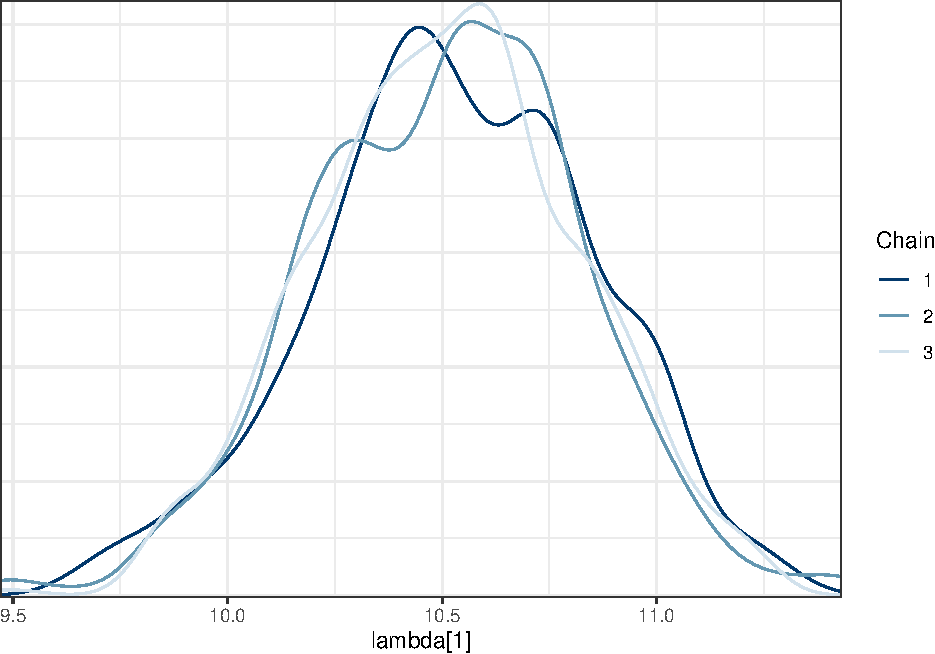
\includegraphics{Vignette_files/figure-latex/unnamed-chunk-15-1.pdf}

\linespread{1}

To see a traceplot for all \(\lambda\) parameters, run the following:

\linespread{1}

\begin{Shaded}
\begin{Highlighting}[]
\NormalTok{bayesplot}\SpecialCharTok{::}\FunctionTok{mcmc\_trace}\NormalTok{(fit\_1\_1, }\AttributeTok{regex\_pars =} \StringTok{"lambda"}\NormalTok{)}
\end{Highlighting}
\end{Shaded}

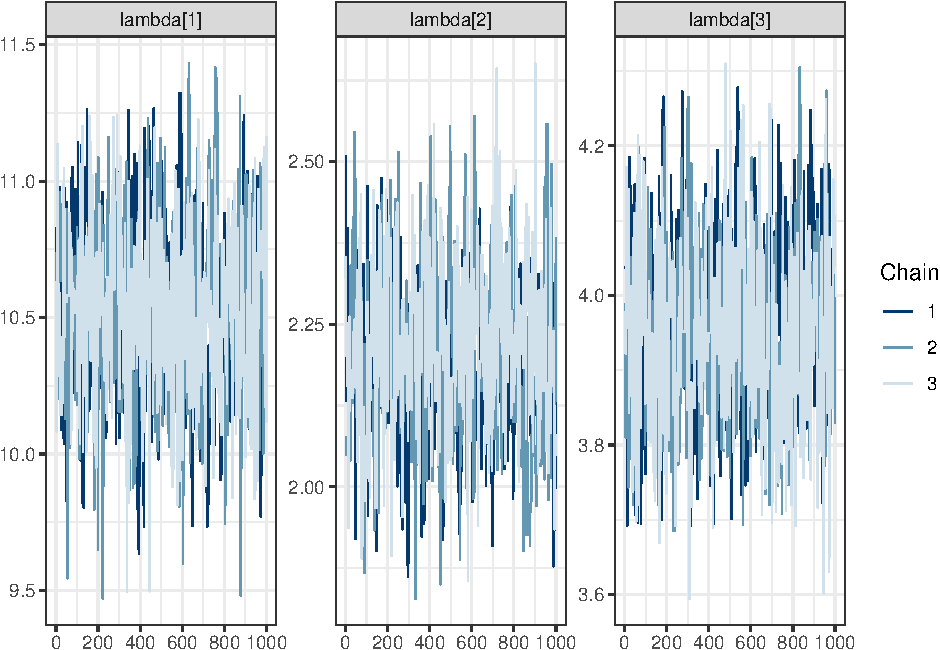
\includegraphics{Vignette_files/figure-latex/unnamed-chunk-16-1.pdf}

\linespread{1}

The Bayesplot package has many other visualizations that are available. See their \href{http://mc-stan.org/bayesplot/}{website} for more examples and details (\url{http://mc-stan.org/bayesplot/}).

The density plots show substantial overlap of the three bell-shaped chains, indicating that the MCMC algorithm has converged. This is further supported by visual inspection of traceplots, which show good mixing. In a simulation study, visual inspection of all traceplots for all parameters in each fitted model is infeasible. Instead, we recommend checking summary tables to make sure that a dataset is included only if all parameters in the model fit to that dataset have Gelman-Rubin statistics \(\hat{R} \leq 1.1.\) This can be achieved using functions from the dplyr package, where we can see that all parameters were below 1.1, in all five datasets under scenarios 1-4 (which are the only ones considered here).

\linespread{1}

\linespread{1}

\linespread{1}

\begin{Shaded}
\begin{Highlighting}[]
\NormalTok{sims\_output }\SpecialCharTok{\%\textgreater{}\%} 
  \FunctionTok{group\_by}\NormalTok{(theta\_scenario, scenario, dataset) }\SpecialCharTok{\%\textgreater{}\%} 
  \FunctionTok{mutate}\NormalTok{(}\AttributeTok{all\_pars\_converged =} \FunctionTok{ifelse}\NormalTok{(}\FunctionTok{unique}\NormalTok{(converge) }\SpecialCharTok{==} \DecValTok{1}\NormalTok{, }\DecValTok{1}\NormalTok{, }\DecValTok{0}\NormalTok{)) }\SpecialCharTok{\%\textgreater{}\%} 
  \FunctionTok{filter}\NormalTok{(all\_pars\_converged }\SpecialCharTok{==} \DecValTok{1}\NormalTok{) }\SpecialCharTok{\%\textgreater{}\%} 
  \FunctionTok{ungroup}\NormalTok{ () }\SpecialCharTok{\%\textgreater{}\%} 
  \FunctionTok{select}\NormalTok{(theta\_scenario, scenario, dataset) }\SpecialCharTok{\%\textgreater{}\%} 
  \FunctionTok{distinct}\NormalTok{()}
\end{Highlighting}
\end{Shaded}

\begin{verbatim}
## # A tibble: 20 x 3
##    theta_scenario scenario dataset
##             <dbl>    <int>   <int>
##  1              1        1       1
##  2              1        1       2
##  3              1        1       3
##  4              1        1       4
##  5              1        1       5
##  6              1        2       1
##  7              1        2       2
##  8              1        2       3
##  9              1        2       4
## 10              1        2       5
## 11              1        3       1
## 12              1        3       2
## 13              1        3       3
## 14              1        3       4
## 15              1        3       5
## 16              1        4       1
## 17              1        4       2
## 18              1        4       3
## 19              1        4       4
## 20              1        4       5
\end{verbatim}

\linespread{1}

Note that the visualization functions described in the next section automatically filter to only include model results if the MCMC algorithm shows evidence of convergence.

\hypertarget{step-6-visualize-simulations}{%
\subsection{Step 6: Visualize simulations}\label{step-6-visualize-simulations}}

Once the simulation study is complete, you can visualize the results using two functions, \texttt{visualize\_parameter\_group} and \texttt{visualize\_single\_parameter}. These functions ensure that only converged models are included in the visualization. \texttt{visualize\_parameter\_group} is useful for examining an entire set of parameters, such as all relative activity parameters. The set of expected inputs for \texttt{visualize\_parameter\_group} are:

\begin{itemize}
\tightlist
\item
  \texttt{sim\_summary}: A dataframe in the format of the summaries output by \texttt{run\_sims}. Column names must match those of the \texttt{run\_sims} output.
\item
  \texttt{pars}: The name of the parameter ``group'' to be visualized (e.g, ``psi'', ``lambda'' or ``theta'').
\item
  \texttt{theta\_scenario}: The \(\Theta\) classifier ID.
\item
  \texttt{scenarios}: Which scenarios to visualize?
\item
  \texttt{convergence\_threshold}: What value should \(\hat{R}\) be below to be considered ``converged''? Default value is 1.1. This value matters because only model fits where all parameter values are below the \texttt{convergence\_threshold} are used for visualization.
\end{itemize}

We can visualize the inference for the relative activity parameters in the first three scenarios in our simulation study above by running the code below. Note that we have set \texttt{convergence\_threshold} to be unrealistically high for illustration purposes. Typically, the default value of 1.1 is as high of an \(\hat{R}\) value as possible for the MCMC chains to be considered ``converged''.

\linespread{1}

\begin{Shaded}
\begin{Highlighting}[]
\FunctionTok{source}\NormalTok{(}\StringTok{"../Summary Figures/visualize\_sims.R"}\NormalTok{)}
\FunctionTok{visualize\_parameter\_group}\NormalTok{(}\AttributeTok{sim\_summary =}\NormalTok{ sims\_output, }
                          \AttributeTok{pars =} \StringTok{"lambda"}\NormalTok{, }
                          \AttributeTok{theta\_scenario =} \DecValTok{1}\NormalTok{, }
                          \AttributeTok{scenarios =} \DecValTok{1}\SpecialCharTok{:}\DecValTok{4}\NormalTok{, }
                          \AttributeTok{convergence\_threshold =} \FloatTok{1.1}\NormalTok{)}
\end{Highlighting}
\end{Shaded}

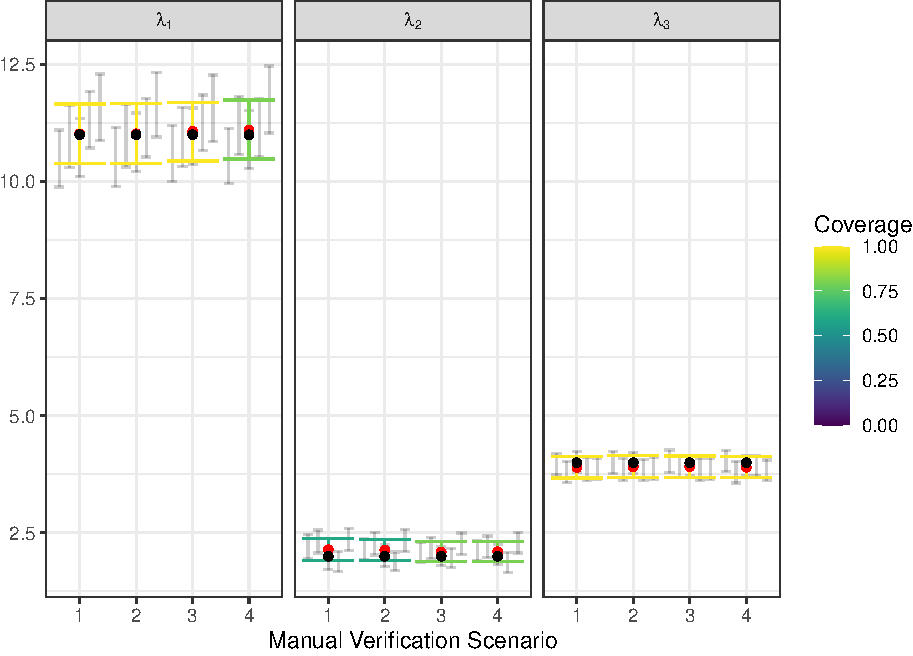
\includegraphics{Vignette_files/figure-latex/unnamed-chunk-19-1.pdf}

\linespread{1}

The features of the plot are as follows:

\begin{itemize}
\tightlist
\item
  Facet grids: parameters
\item
  X-axis: Manual verification scenario
\item
  y-axis: parameter values
\item
  Small grey error bars: 95\% posterior interval for an individual model fit where all parameters were below \texttt{convergence\_threshold}.
\item
  Colored error bars: average 95\% posterior interval across all converged models under that scenario.
\item
  Color: Coverage, or the rate at which 95\% posterior intervals contain the true data-generating parameter value.
\item
  Black dots: the true value of the parameter
\item
  Red dots: average posterior mean
\end{itemize}

If you would like to visualize a single parameter, use \texttt{visualize\_single\_parameter}, which takes the same arguments as the previous visualization function:

\linespread{1}

\begin{Shaded}
\begin{Highlighting}[]
\CommentTok{\# note the space between the indices for theta[2, 1]}
\FunctionTok{visualize\_single\_parameter}\NormalTok{(sims\_output, }\AttributeTok{par =} \StringTok{"theta[2, 1]"}\NormalTok{, }
                           \AttributeTok{theta\_scenario =} \DecValTok{1}\NormalTok{, }
                           \AttributeTok{scenarios =} \DecValTok{1}\SpecialCharTok{:}\DecValTok{3}\NormalTok{, }
                           \AttributeTok{convergence\_threshold =} \FloatTok{1.2}\NormalTok{)}
\end{Highlighting}
\end{Shaded}

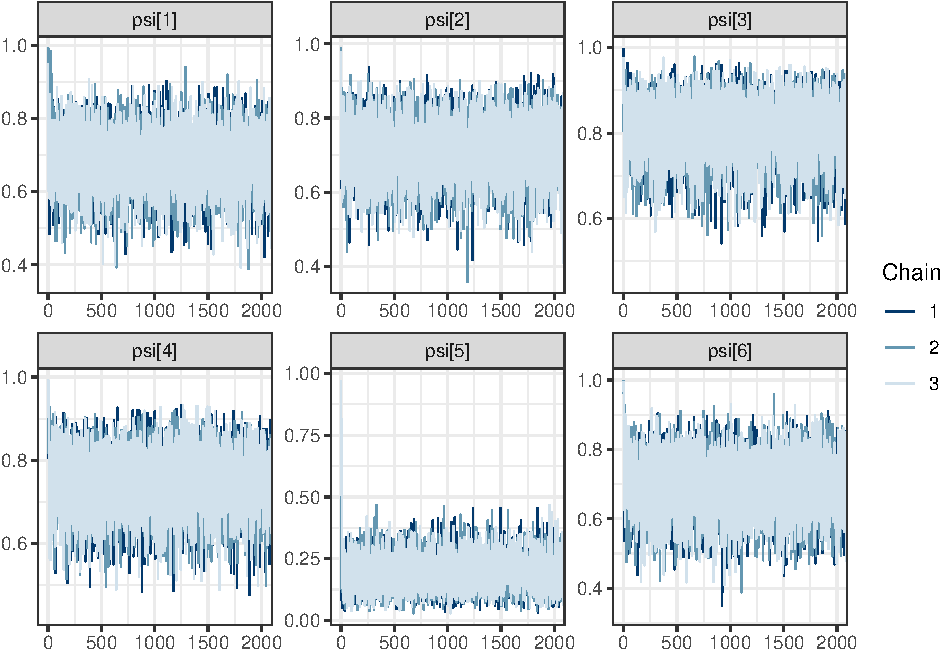
\includegraphics{Vignette_files/figure-latex/unnamed-chunk-20-1.pdf}

\linespread{1}

Note that the scale of the y-axis is free to change from one visualization to the next. Additionally, if no datasets show evidence of convergence (i.e., no fitted models have \(\hat{R} \leq c\) for all parameters, where \(c\) is the specified convergence threshold) under a given scenario, the scenario will not appear on the x-axis.

\hypertarget{FEexample}{%
\section{Example: simulations with a fixed-effort design}\label{FEexample}}

The previous section outlined the mechanics of using the functions contained in the ValidationExplorer repo. Here, we provide a streamlined example with a fixed-effort validation design, and emphasize how the tool may be used to aid the decision process about the appropriate level of effort for reliable inference. Our example uses the second validation design available in the ValidationExplorer: a fixed-effort design. Under this validation design, a random sample of \(p\) percent of all recordings is taken from the first detector night at each site, where \(p\) is specified by the user.

We begin the simulation process by selecting the occurrence probabilities \(\psi_k\) and relative activity rates \(\lambda_k\) for each species \(k\). We must also specify the assumed classification probabilities.

If estimates exist for the species of interest, one option could be to adopt those. For instance, if we assumed an assemblage comprised of \emph{Eptesicus fuscus} (EPFU)\emph{, Lasiurus cinereus} (LACI)\emph{, Lasinoycteris noctivagans} (LANO), and \emph{Myotis lucifugus} (MYLU), we could use posterior estimates obtained by Stratton et al. (2022). These are shown in Table 1.

\begin{table}
  \centering
  \begin{tabular} {ccc}
    \toprule 
    Species & $\psi$ & $\lambda$ \\ 
    \midrule
    EPFU    & 0.633  & 5.934 \\
    LACI    & 0.612  & 4.160 \\
    LANO    & 0.849  & 14.25 \\
    MYLU    & 0.898  & 28.25 \\
    \bottomrule
  \end{tabular}
  \caption{Posterior estimates obtained by Stratton et al., (2022)}
  \label{parVals}
\end{table}

The classification matrix estimated by Stratton et al. (2022) was for an assemblage of 11 species, and due to the sum-to-one constraint on the rows, values cannot be borrowed directly. However, we might use these to choose realistic values, starting with the diagonal entries: \[\Theta = \begin{bmatrix}
  0.788 & & &\\
   & 0.983 & &\\
   & & 0.983 & \\
   & & & 0.965 \\
\end{bmatrix}.\]

A strategy for filling in off-diagonal entries could be to use the estimates from Stratton et al. (2022) and augment each value by the difference between each row sum and 1, divided by the number species. For example, we might fill in the first row with the estimates from Stratton et al. (2022):

\[\Theta = \begin{bmatrix}
  0.7878 & 0.176 & 0.0245 & 0.0014 \\
  0.0090 & 0.9826 & 0.0018 & 0.0009 \\
  0.0071 & 0.0051 & 0.9829 & 0.0028 \\
  0.0002 & 0.0003 & 0.0002 & 0.9650 \\
\end{bmatrix}.\]

However, the first row sums to 0.788 + 0.176 + 0.0245 + 0.0014 \(\approx\) 0.99. The remaining 0.01 can be divided by four and added to each entry, so that the first row of \(\Theta\) is now \((0.7905, 0.1785, 0.027, 0.0039).\) This process can be repeated to obtain an empirically-informed classification matrix. Alternatively, simulated matrices can be simulated using the same procedure as \texttt{test\_theta2} (Section \ref{dataSimulation}). Using this procedure, one must ensure the entries of the matrix in the first argument of \texttt{apply} are adjusted to yield classification matrices that align with expert opinions.

With the parameter values chosen, we begin data simulation. Note that the \texttt{scenarios} argument is now a vector, in contrast with the proceeding example.

\linespread{1}

\begin{Shaded}
\begin{Highlighting}[]
\NormalTok{psi }\OtherTok{\textless{}{-}} \FunctionTok{c}\NormalTok{(}\FloatTok{0.633}\NormalTok{, }\FloatTok{0.612}\NormalTok{, }\FloatTok{0.849}\NormalTok{, }\FloatTok{0.898}\NormalTok{)}
\NormalTok{lambda }\OtherTok{\textless{}{-}} \FunctionTok{c}\NormalTok{(}\FloatTok{5.934}\NormalTok{, }\FloatTok{4.160}\NormalTok{, }\FloatTok{14.25}\NormalTok{, }\FloatTok{28.25}\NormalTok{)}

\NormalTok{Theta\_FE }\OtherTok{\textless{}{-}} \FunctionTok{matrix}\NormalTok{(}
  \FunctionTok{c}\NormalTok{(}
    \FloatTok{0.7905}\NormalTok{, }\FloatTok{0.1785}\NormalTok{, }\FloatTok{0.027}\NormalTok{, }\FloatTok{0.0039}\NormalTok{, }
    \FloatTok{0.010425}\NormalTok{, }\FloatTok{0.984025}\NormalTok{, }\FloatTok{0.00322}\NormalTok{, }\FloatTok{0.002325}\NormalTok{, }
    \FloatTok{0.007625}\NormalTok{, }\FloatTok{0.005625}\NormalTok{, }\FloatTok{0.983425}\NormalTok{, }\FloatTok{0.003325}\NormalTok{,}
    \FloatTok{0.008775}\NormalTok{, }\FloatTok{0.008875}\NormalTok{, }\FloatTok{0.008775}\NormalTok{, }\FloatTok{0.973575}
\NormalTok{  ), }
  \AttributeTok{nrow =} \DecValTok{4}\NormalTok{, }
  \AttributeTok{byrow =} \ConstantTok{TRUE}
\NormalTok{)}

\NormalTok{nsites }\OtherTok{\textless{}{-}} \DecValTok{100}
\NormalTok{nvisits }\OtherTok{\textless{}{-}} \DecValTok{4}
\NormalTok{nspecies }\OtherTok{\textless{}{-}} \FunctionTok{length}\NormalTok{(psi)}

\NormalTok{FE\_data }\OtherTok{\textless{}{-}} \FunctionTok{simulate\_validatedData}\NormalTok{(}
  \AttributeTok{n\_datasets =} \DecValTok{5}\NormalTok{, }
  \AttributeTok{validation\_design =} \StringTok{"FixedPercent"}\NormalTok{,}
  \AttributeTok{scenarios =} \FunctionTok{c}\NormalTok{(}\FloatTok{0.05}\NormalTok{, .}\DecValTok{25}\NormalTok{,  }\FloatTok{0.5}\NormalTok{, }\FloatTok{0.75}\NormalTok{), }\CommentTok{\# Note the vector of possible scenarios}
  \AttributeTok{nsites =}\NormalTok{ nsites, }
  \AttributeTok{nvisits =}\NormalTok{ nvisits, }
  \AttributeTok{nspecies =}\NormalTok{ nspecies,}
  \AttributeTok{psi =}\NormalTok{ psi, }
  \AttributeTok{lambda =}\NormalTok{ lambda,}
  \AttributeTok{theta =}\NormalTok{ Theta\_FE, }
  \AttributeTok{save\_datasets =} \ConstantTok{TRUE}\NormalTok{,}
  \AttributeTok{save\_masked\_datasets =} \ConstantTok{TRUE}\NormalTok{,}
  \AttributeTok{directory =} \FunctionTok{paste0}\NormalTok{(here}\SpecialCharTok{::}\FunctionTok{here}\NormalTok{(}\StringTok{"Testing"}\NormalTok{, }\StringTok{"FixedEffortExample"}\NormalTok{))}
\NormalTok{)}
\end{Highlighting}
\end{Shaded}

\linespread{1}

Next, we fit the model to the simulated data:

\linespread{1}

\begin{Shaded}
\begin{Highlighting}[]
\NormalTok{FE\_model\_fits }\OtherTok{\textless{}{-}} \FunctionTok{run\_sims}\NormalTok{(}
  \AttributeTok{data\_list =}\NormalTok{ FE\_data}\SpecialCharTok{$}\NormalTok{masked\_dfs,}
  \AttributeTok{zeros\_list =}\NormalTok{ FE\_data}\SpecialCharTok{$}\NormalTok{zeros, }
  \AttributeTok{theta\_scenario\_id =} \DecValTok{1}\NormalTok{,}
  \AttributeTok{save\_fits =} \ConstantTok{FALSE}\NormalTok{,}
  \AttributeTok{DGVs =} \FunctionTok{list}\NormalTok{(}\AttributeTok{lambda =}\NormalTok{ lambda, }\AttributeTok{psi =}\NormalTok{ psi, }\AttributeTok{theta =}\NormalTok{ Theta\_FE),}
  \AttributeTok{save\_individual\_summaries\_list =} \ConstantTok{FALSE}\NormalTok{,}
  \AttributeTok{directory =} \FunctionTok{here}\NormalTok{(}\StringTok{"Testing"}\NormalTok{, }\StringTok{"FixedEffortExample"}\NormalTok{)}
\NormalTok{)}
\end{Highlighting}
\end{Shaded}

\linespread{1}

We can visualize the results from the model for each parameter group:

\linespread{1}

\linespread{1}

\linespread{1}

\begin{Shaded}
\begin{Highlighting}[]
\FunctionTok{visualize\_parameter\_group}\NormalTok{(FE\_model\_fits, }\AttributeTok{pars =} \StringTok{"lambda"}\NormalTok{, }\AttributeTok{theta\_scenario =} \DecValTok{1}\NormalTok{, }\AttributeTok{scenarios =} \DecValTok{1}\SpecialCharTok{:}\DecValTok{4}\NormalTok{)}
\end{Highlighting}
\end{Shaded}

\begin{figure}
\centering
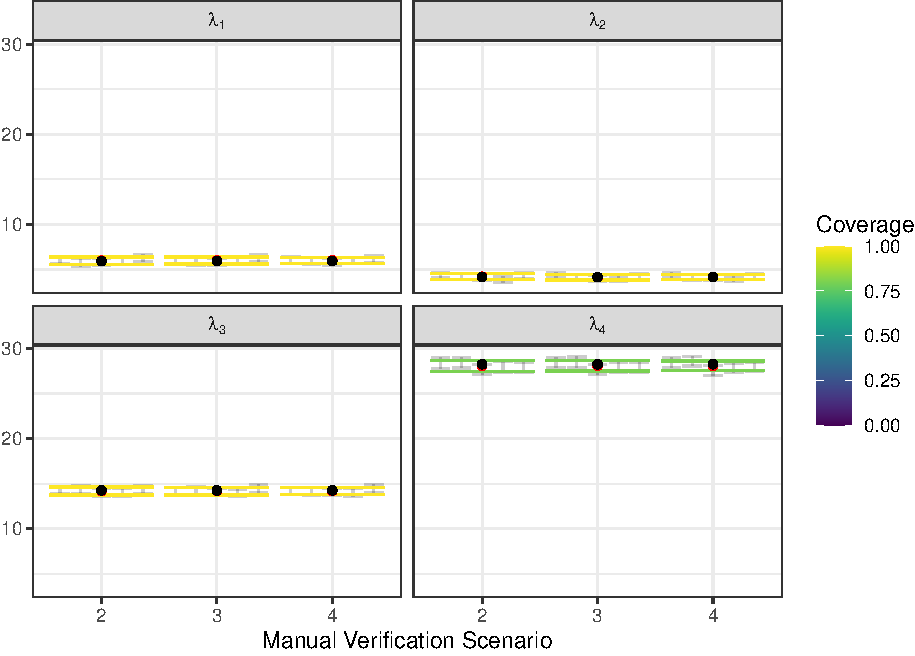
\includegraphics{Vignette_files/figure-latex/FElambda-1.pdf}
\caption{\label{fig:FElambda}Simulation study results for relative activity parameters under a fixed effort design. The percentages corresponding to the manual verification scenarios are given in the call to simulate\_validatedData.}
\end{figure}

\linespread{1}

The first fixed effort design, where 5\% of all recordings from the first detector-night at each site were validated, did not provide enough information for any models fit to the simulated data sets to have \(\hat{R} \leq 1.1\) for all parameters after 2000 MCMC iterations. This is evident in Figure \ref{fig:FElambda} -- the first manual verification scenario is missing from the \(x\)-axis. For all other validation scenarios, all parameters in all models converged, as evidenced by the presence of five grey intervals in the background for each parameter-scenario combination. Based on the absence of a red point for any relative activity parameter in any of the validation scenarios, minimal estimation error is expected for relative activity under validation scenarios 2-4. For species 1-3 (i.e., EPFU, LACI, and LANO), the figure shows high coverage of relative activity parameters (\(\lambda_1, \lambda_2 \text{ and } \lambda_3\) in Figure \ref{fig:FElambda}). Coverage is slightly low for species 4 (MYLU), but this is likely due to only five datasets being fit for this vignette -- if one 95\% posterior interval fails to capture the true parameter value, coverage is reduced to 80\%, as in Figure \ref{fig:FElambda}. When using our software tool for evaluating management decisions, we recommend fitting models to at least 50-100 datasets to ensure that estimates of long-run behavior (e.g., coverage or expected estimation error) are reliable. Note that depending on the size of the species assemblage and the parameter settings, simulation studies could be time-cosuming and plan accordingly.

\linespread{1}

\begin{Shaded}
\begin{Highlighting}[]
\FunctionTok{visualize\_parameter\_group}\NormalTok{(FE\_model\_fits, }\AttributeTok{pars =} \StringTok{"psi"}\NormalTok{, }\AttributeTok{theta\_scenario =} \DecValTok{1}\NormalTok{, }\AttributeTok{scenarios =} \DecValTok{1}\SpecialCharTok{:}\DecValTok{4}\NormalTok{)}
\end{Highlighting}
\end{Shaded}

\begin{figure}
\centering
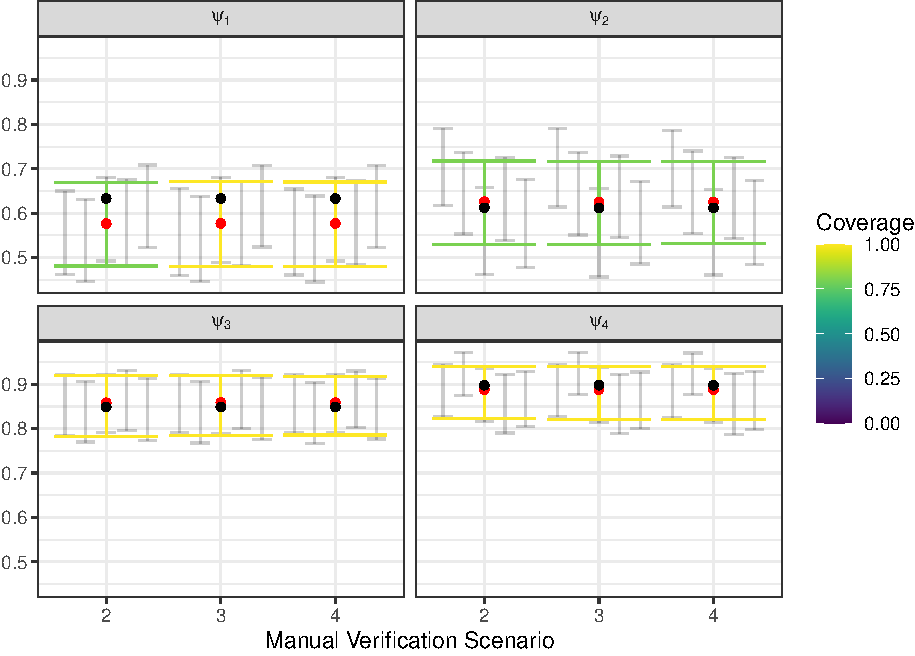
\includegraphics{Vignette_files/figure-latex/FEpsi-1.pdf}
\caption{\label{fig:FEpsi}Simulation study results for occurrence probabilities under a fixed effort design.}
\end{figure}

\linespread{1}

The simulation results for \(\psi_k\) exhibits similar characteristics to Figure \ref{fig:FElambda}, especially with regard to convergence of MCMC algorithms (Figure \ref{fig:FEpsi}). However, we may expect slightly higher estimation error, especially for \(\psi_1\), which is the occurrence probability of EPFU. This estimation error does not appear to change across the various validation scenarios. However, coverage for \(\psi_1\) improves with greater validation effort (coverage = 80\% in scenario 2, but is 100\% in scenario 3). Coverage is slightly low for \(\psi_2\) across all validation scenarios. Again, these results may change when a greater number of datasets are used for the simulations, which warrants follow-up. If results remain the same after fitting models to 50 or more datasets, one might consider leaning towards validation scenario 3 based on the simulation results for \(\psi_1\).

\linespread{1}

\begin{Shaded}
\begin{Highlighting}[]
\FunctionTok{visualize\_parameter\_group}\NormalTok{(FE\_model\_fits, }\AttributeTok{pars =} \StringTok{"theta"}\NormalTok{, }\AttributeTok{theta\_scenario =} \DecValTok{1}\NormalTok{, }\AttributeTok{scenarios =} \DecValTok{1}\SpecialCharTok{:}\DecValTok{4}\NormalTok{)}
\end{Highlighting}
\end{Shaded}

\begin{figure}
\centering
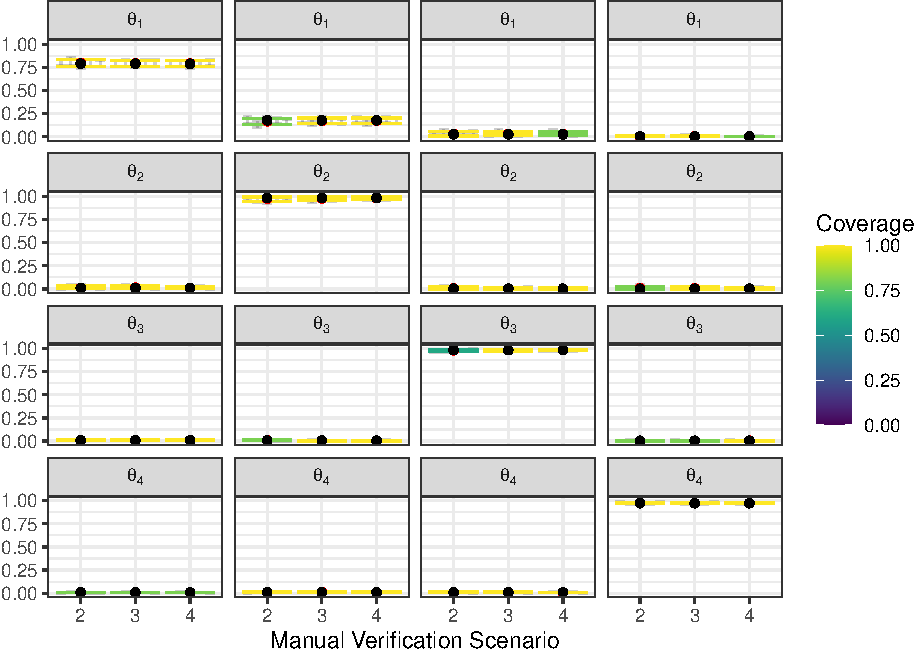
\includegraphics{Vignette_files/figure-latex/FEtheta-1.pdf}
\caption{\label{fig:FEtheta}Simulation study results for classification parameters under a fixed effort design.}
\end{figure}

\linespread{1}

The simulation results for the classification matrix shown in Figure \ref{fig:FEtheta} further support validation scenario 3. Typically, the misclassification parameters in the \(\Theta\) matrix are regarded as nuisance parameters. However, reliable inference for all parameters is desireable, and Figure \ref{fig:FEtheta} further suggests that the 3rd validation scenario may be the best option. Often, this level of validation effort leads to near-nominal coverage of 95\% posterior intervals and minimal estimation error, but requires fewer recordings be validated than validation scenario 4. The exceptions are \(\theta_{34}\) (third row, fourth column) and \(\theta_{41}\) (fourth row, first column), which have coverage slightly below nominal levels under validation scenario 3 (Figure \ref{fig:FEtheta}). as noted above this is likely an artifact of the very small number of datasets used in this example.

We can examine the expected number of validated recordings (for this species assemblage) using the \texttt{summarize\_n\_validated} function:

\linespread{1}

\begin{Shaded}
\begin{Highlighting}[]
\FunctionTok{summarize\_n\_validated}\NormalTok{(FE\_data}\SpecialCharTok{$}\NormalTok{masked\_dfs)}
\end{Highlighting}
\end{Shaded}

\begin{verbatim}
## [1]  268.0 1134.6 2218.0 3327.2
\end{verbatim}

\linespread{1}

If the decision is made to use a fixed-effort design, with the third level of validation effort investigated in these scenarios, then around 2200 recordings will need to be validated. If this is infeasible, additional simulations could be undertaken to fine-tune the validation effort to a lower level (somewhere between validation scenario 2 and validation scenario 3) while also ensuring near nominal coverage and minimal estimation error.

\hypertarget{conclusion}{%
\section{Conclusion}\label{conclusion}}

We have demonstrated the use of the ValidationExplorer software tool through two examples. Note that with any simulation study, including those conducted using the ValidationExplorer, results are conditional on the settings and assumptions. In the case of the count-detection model framework, the assumptions are

\begin{itemize}
\tightlist
\item
  The occurrence of species within a site are independent; the presence of one species carries no information about the presence or absence of another.
\item
  For any one species, its occurrence at one location is independent of its occurrence at any other location (independence across sites).
\item
  Visits to a site (i.e., detector nights) are independent.
\item
  Recordings within the same site-visit are independent. This holds regardless of whether a recording is validated or remains ambiguous (only has an autoID label).
\item
  The count of recordings generated by a species in a single detector night is a Poisson random variable.
\end{itemize}

\noindent The settings include the number of datasets used in the simulations, the assumed characteristics of the species assemblage (i.e., the values for each \(\psi_k\) and \(\lambda_k\)) and classifier (\(\Theta\)), and the number of sites and visits. Our hope is that the ValidationExplorer provides a useful tool for assessing the merits of various validation designs, so that effort can be thoughtfully assigned based on program goals and monitoring objectives. Ultimately, we hope that this software streamlines the bat acoustic workflow and allows for efficient processing of information.

\hypertarget{references}{%
\section*{References}\label{references}}
\addcontentsline{toc}{section}{References}

\hypertarget{refs}{}
\begin{CSLReferences}{1}{0}
\leavevmode\vadjust pre{\hypertarget{ref-nimble}{}}%
de Valpine, Perry, Christopher Paciorek, Daniel Turek, Nick Michaud, Cliff Anderson-Bergman, Fritz Obermeyer, Claudia Wehrhahn Cortes, Abel Rodrìguez, Duncan Temple Lang, and Sally Paganin. 2022. \emph{{NIMBLE} User Manual} (version 0.12.2). \url{https://doi.org/10.5281/zenodo.1211190}.

\leavevmode\vadjust pre{\hypertarget{ref-irvine22}{}}%
Irvine, Kathryn M., Katharine M. Banner, Christian Stratton, William M. Ford, and Brian E. Reichert. 2022. {``Statistical Assessment on Determining Local Presence of Rare Bat Species.''} \emph{Ecology}.

\leavevmode\vadjust pre{\hypertarget{ref-loeb15}{}}%
Loeb, Susan C., Thomas J. Rodhouse, Laura E. Ellison, Cori L. Lausen, Jonathan D. Reichard, Kathryn M. Irvine, Thomas E. Ingersoll, et al. 2015. {``A Plan for the {N}orth {A}merican Bat Monitoring Program ({NAB}at).''} SRS-208. USDA Forest Service.

\leavevmode\vadjust pre{\hypertarget{ref-rubin76}{}}%
Rubin, Donald B. 1976. {``Inference and Missing Data.''} \emph{Biometrika} 63 (3): 581--92. \url{http://www.jstor.org/stable/2335739}.

\leavevmode\vadjust pre{\hypertarget{ref-stratton22}{}}%
Stratton, Christian, Kathryn M. Irvine, Katharine M. Banner, Wilson J. Wright, Cori Lausen, and Jason Rae. 2022. {``Coupling Validation Effort with in Situ Bioacoustic Data Improves Estimating Relative Activity and Occupancy for Multiple Species with Cross-Species Misclassifications.''} \emph{Methods in Ecology and Evolution} 13 (6): 1288--1303. https://doi.org/\url{https://doi.org/10.1111/2041-210X.13831}.

\leavevmode\vadjust pre{\hypertarget{ref-nimblejournal}{}}%
Valpine, Perry de, Daniel Turek, Christopher J. Paciorek, Clifford Anderson-Bergman, Duncan Temple Lang, and Rastislav Bodik. 2017. {``Programming {W}ith {M}odels: {W}riting {S}tatistical {A}lgorithms for {G}eneral {M}odel {S}tructures {W}ith {NIMBLE}.''} \emph{Journal of {C}omputational and {G}raphical {S}tatistics} 26 (2): 403--13. \url{https://doi.org/10.1080/10618600.2016.1172487}.

\leavevmode\vadjust pre{\hypertarget{ref-wright20}{}}%
Wright, Wilson J., Kathryn M. Irvine, Emily S. Almberg, Andrea R. Litt, and Nigel Yoccoz. 2020. {``Modelling Misclassification in Multi‐species Acoustic Data When Estimating Occupancy and Relative Activity.''} \emph{Methods in Ecology and Evolution} 11 (1): 71--81.

\end{CSLReferences}

\end{document}
